\section{Results}

Implementation of the our approach is provided in the \texttt{R} package \href{https://dajmcdon.github.io/rtestim/}{\texttt{rtestim}}. 


\subsection{Experimental settings}

% problem settings
%% Rt
We consider four scenarios of the time-varying effective reproduction numbers to simulate different epidemics. The first two scenarios are simple cases that are rapidly controlled by intervention, where the graphical curves consist of one knot and two segments. Scenario 1 is instantaneous prior and post-intervention, and Scenario 2 is exponentially grow and decay. The last two scenarios are more complicated, where more waves in the epidemics are involved. Scenario 3 has four linear segments with three knots, which reflect the effect of intervention, the resurgence to large epidemics, and the suppression of pandemic respectively. Scenario 4 involves more complicated waves and curvatures of the epidemic. Effective reproduction numbers across all scenarios are evenly spaced. 
% motivation
The first three scenarios and the last scenario are motivated by \cite{parag2021improved, gressani2022epilps} respectively. 
% name the scenarios
We name the four scenarios as (1) 2-segment constant line, (2) 2-segment exponential curve, (3) 4-segment linear line, and (4) periodic curve respectively. 

We consider epidemics of length $n=300$. 
Specifically, in Scenario 1, $\calR_t = 2, 0.8$ before and after $t=70$. In Scenario 2, $\calR_t$ increases and decreases exponentially with rates $0.015, 0.005$ pre and post $t=50$. In Scenario 3, $\calR_t$ reduces from $2.5$ to $2$ linearly between $t\in[1,60]$, falls to $0.8$ at $t=61$ and goes linearly down to $0.6$ until $t=110$, resurges to $1.7$ at $t=111$ and grows linearly back to $2$ until $t=150$, and then drops to $0.9$ at $t=151$ and descends to $0.5$ until the end. In Scenario 4, $\calR_t$ is a continuous, periodic curve generated by the function $f(x) = 0.2 \lr{ \lr{\sin(\frac{\pi x}{12}) + 1} + \lr{2 \sin\lr{\frac{\pi x}{6}} + 2} + \lr{3 \sin(\frac{\pi x}{1.2}) + 3} }$ at equally spaced points $x\in [0,10]$. 


%% other problem settings
We assume that the serial interval follows Gamma distribution with fixed shapes and scales $(3,3)$, $(2.5,2.5)$, $(3.5,3.5)$ and $(3.5,3.5)$ for Scenarios $1-4$ respectively. We consider all epidemics starting from $N_1=2$ incidences and generating until timepoints $t=300$. We compute the expected incidence $N_t$ use renewal equation, and generate the incidence samples from the Poisson distribution $y_t\sim Pois(N_t)$. 
To verify the performance of our model under the violation of distributional assumption of incidence, we generate incidence samples using negative Binomial distribution with dispersion size 5, i.e., $y_t\sim NB(N_t, {size=}5)$. We generate 50 random samples for each setting of experiments. It results in $4\ \calR_t$ scenarios $\times 2$ Incidences distributions $\times 50$ random samples $= 400$ problems in total. 
Examples of each effective reproduction number scenario with corresponding Poisson and negative Binomial incidences are displayed in \autoref{fig:samples}. 
\begin{figure}[tb]
    \centering
    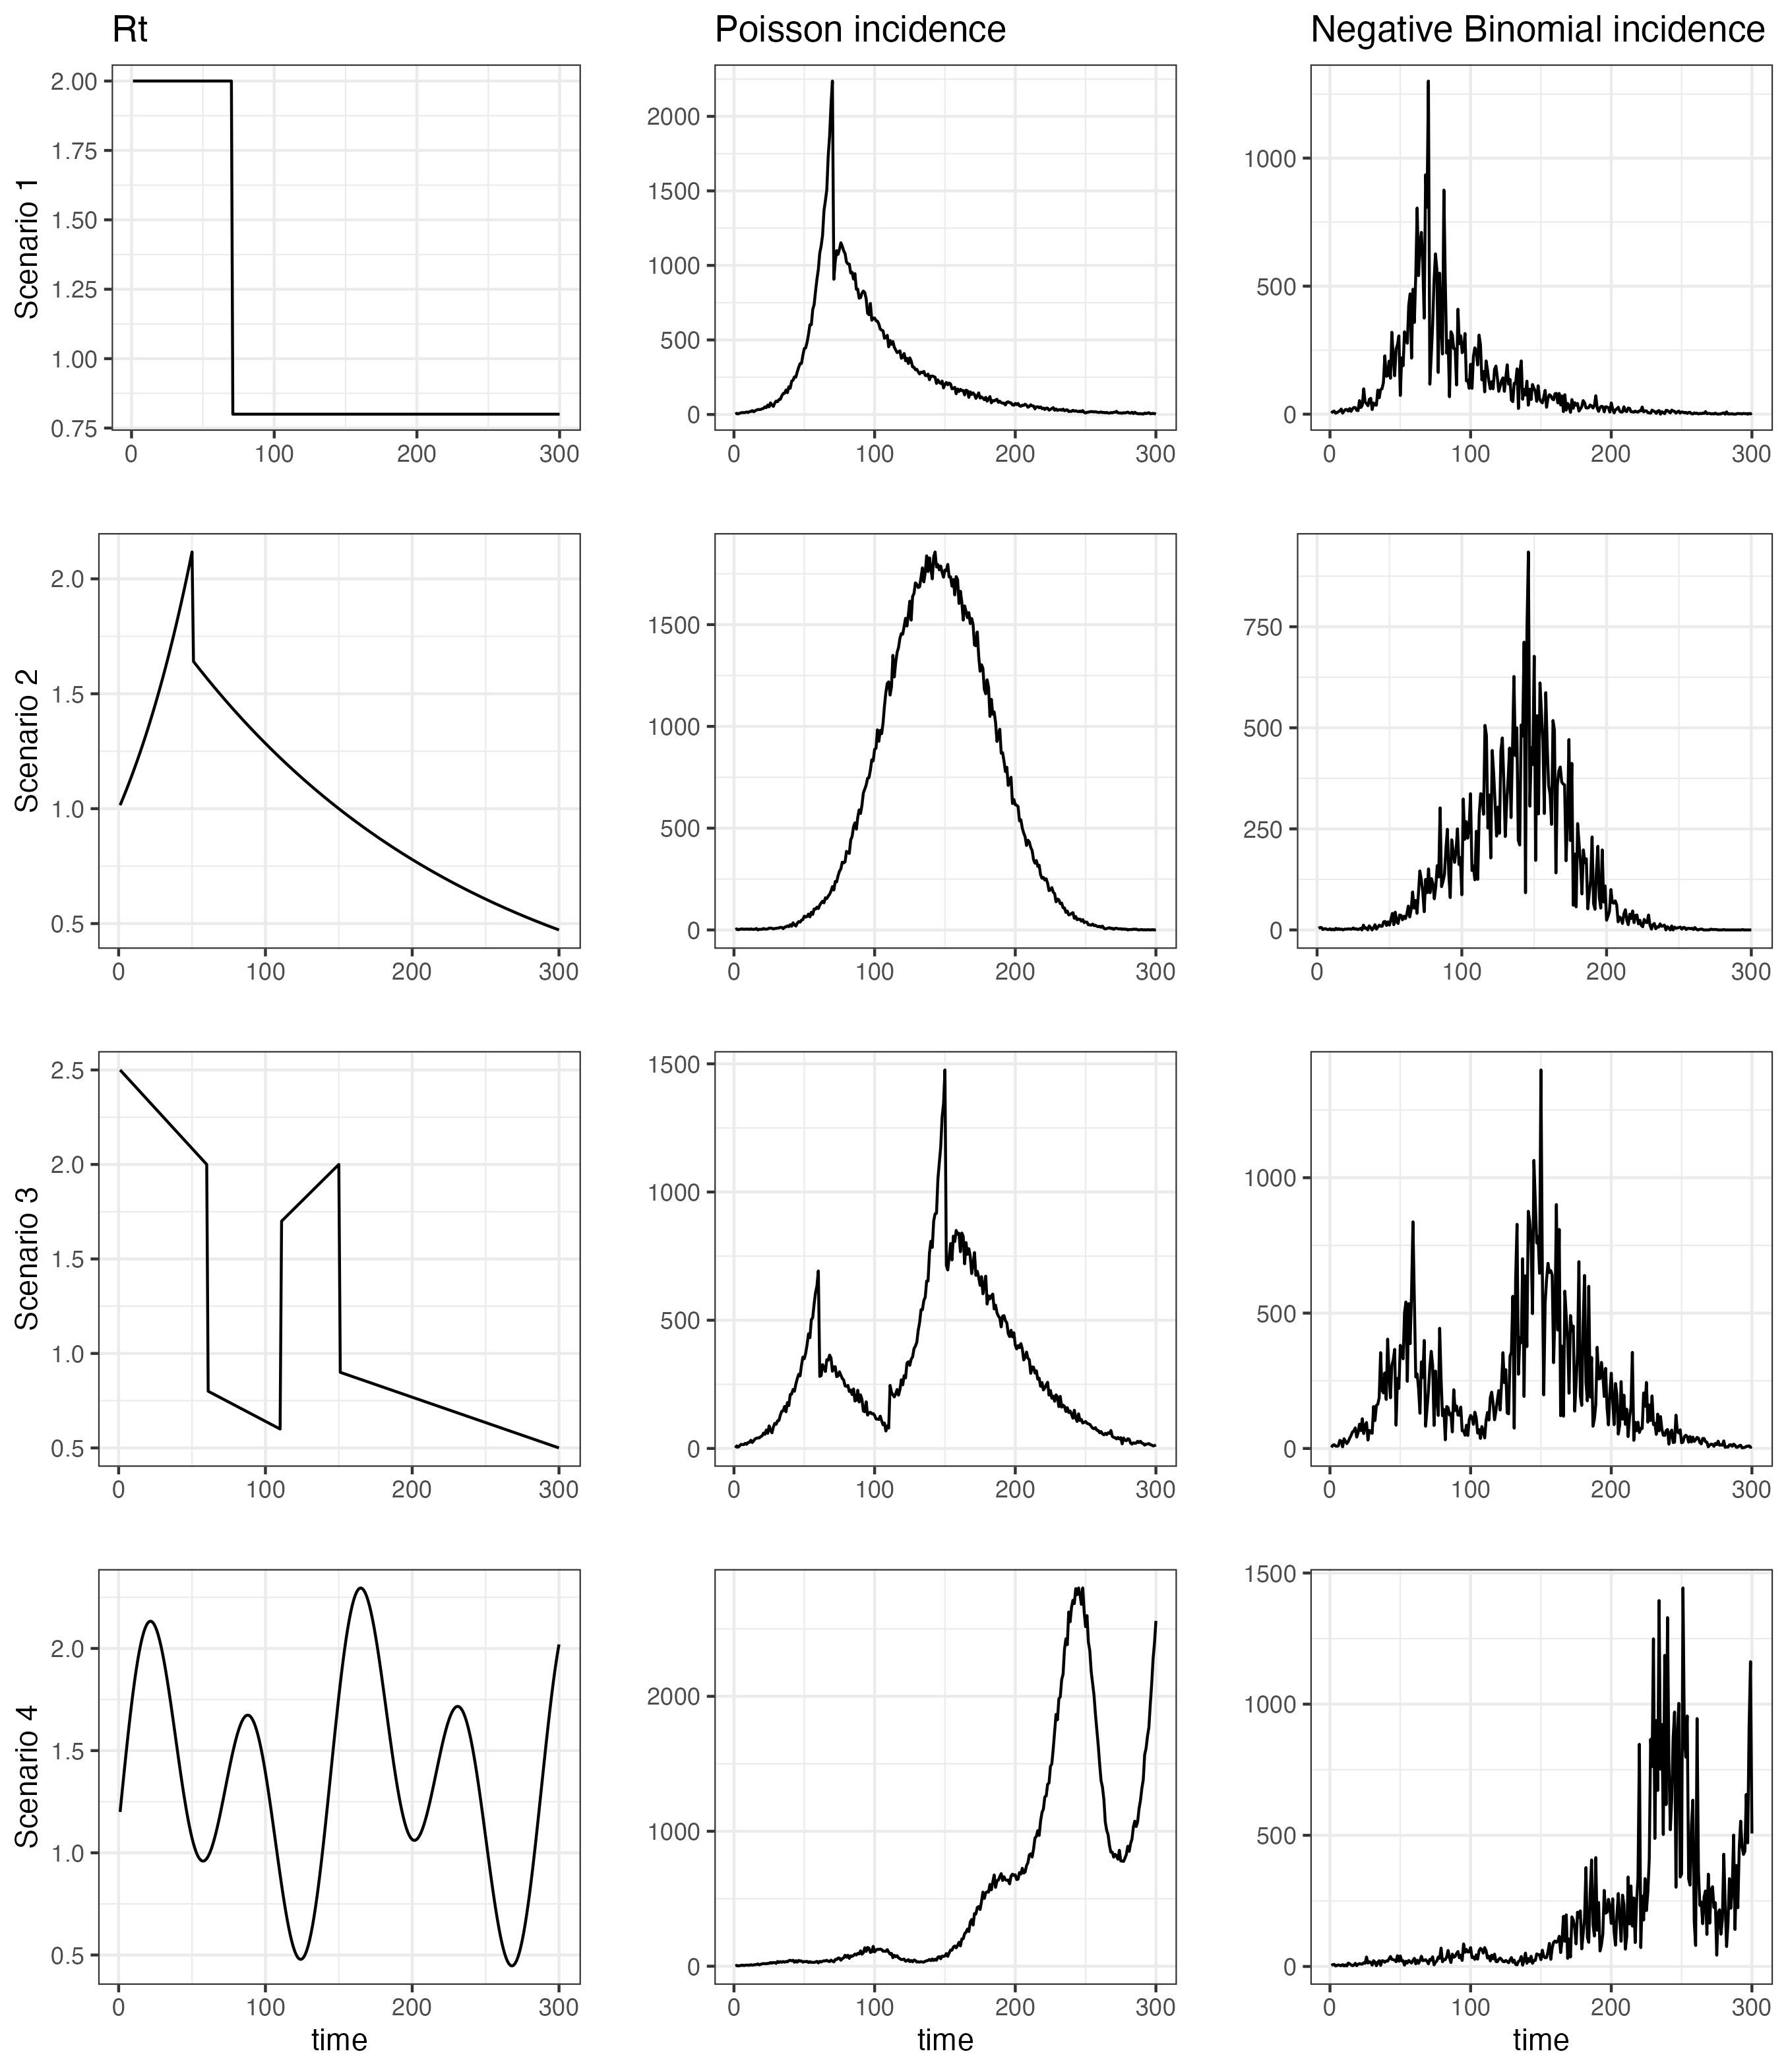
\includegraphics[width=140mm]{fig/plot_samples.png}
    \caption{An example of effective reproduction numbers and corresponding incidences following Poisson or negative Binomial distribution. Three columns illustrate four $\calR_t$ cases, Poisson incidences, and negative Binomial distributed incidences for each $\calR_t$ case respectively. Four rows correspond to four $\calR_t$ cases respectively.} 
    \label{fig:samples}
\end{figure}

% algorithm settings
%% competitors and their settings
We compare our \RtEstim\ to \EpiEstim\ and \EpiLPS. \EpiEstim\ is a widely used Bayesian method that estimates the posterior distribution of effective reproduction numbers given the Gamma prior and Poisson distributed incidences. They estimate the reproduction number over a sliding window by assuming the reproduction number is constant during the specific time window. A longer sliding window averages out more fluctuations and noises, and leads to smoother estimation over time; whereas, a shorter sliding window is more responsive to sudden spikes or declines in a shorter period. We use the default weekly sliding window for the experimental study. Monthly sliding window is also considered in simulation. Since neither of the two sliding windows considerably outperforms the other across all scenarios, we defer the estimation of monthly sliding window to the supplementary document. 
\EpiLPS\ is another Bayesian approach that estimates P-splines coupled with Laplace approximations of the conditional posterior of the spline vector based on negative Binomial distributed incidences. 
%% our RtEstim
We tune the model over the candidate set of size 50 using cross validation. For four scenarios, we estimate piecewise constant $k=0$, piecewise cubic $k=3$, piecewise linear $k=1$ and piecewise cubic polynomials respectively. 
% for all models
We assume the serial intervals are known and use same serial intervals across all models for each problem. 

% KL for exponential family: 
The accuracy of $\calR_t$ estimates is measured by the mean Kullback-Leibler (KL) divergence for Poisson distributions  $$\frac{1}{n} D_{KL}(\hat{\calR}|| \calR) = \frac{1}{n}\sum_{t=1}^n \hat{\calR}_t \log\left(\frac{\hat{\calR}_t}{\calR_t}\right) + {\calR}_t - \hat{\calR}_t,$$ 
where $\calR := \left\{ \calR_t \right\}_{t=1}^n$. %It coincides with the Bregman distance $D_{KL}(\theta_0 || \theta_1) = \varphi(\theta_1) - \varphi(\theta_0) - (\theta_1 - \theta_0)^{\top} \varphi'(\theta_0)$, where $\theta_0,\theta_1$ are natural parameters of the same kind of exponential-family distributions \citep{sadhanala2022exponential}. 
In comparison of the accuracy across methods, we drop the estimates during the first week as the $\calR_t$ estimates of \EpiEstim\ starts at $t=8$. We avoid using the Euclidean ($\ell_2$) norm in favor of KL divergence because Poisson distribution corresponds to points on a discrete lattice, which can be regarded as lying on a curved (non-Euclidean) space in the context of geometry. 
%For negative Binomial cases, we use KL divergence to measure the distances between negative Binomial distributions given the %dispersion rate $\phi$, i.e., 
%\begin{align*}
%    \frac{1}{n} D^{\ast}_{KL}\lr{\hat{\calR}|| \calR} = \frac{1}{n}\sum_{t=1}^n \hat{\calR}_t \log \left(\frac{\hat{\calR}_t}%{\calR_t}\right) + \lr{\hat{\calR}_t + \phi} \log\lr{\frac{\hat{\calR}_t + \phi}{\calR_t + \phi}}. 
%\end{align*}
Other details of the experimental settings are deferred to the supplementary document. 

%\subsubsection*{Cross Validation}
We run leave-third-out cross validation (CV) to choose the best tuning parameter from the candidate set of size $50$, i.e., $\boldsymbol{\lambda} = \{\lambda_1, \cdots, \lambda_{50}\}$. Specifically, we divide the all samples into three folds and build models on each sample set which excludes one fold of the samples across all hyperparameters. Every third samples are placed into the same fold by excluding the first and last samples. We select the tuning parameter that gives the lowest averaged mean squared errors (MSEs) of the estimated reproduction numbers from the observed samples across all folds. 
The experiments are run in \texttt{R} with version 4.3.1 on a MacBook with an Apple M1 Pro chip and RAM 32GB running under macOS Sonoma 14.0. The \texttt{R} packages are of versions \texttt{EpiEstim\_2.2-4}, \texttt{EpiLPS\_1.2.0} and \texttt{rtestim\_0.0.3}. 

\subsection{Experimental results}

% experiment results
\autoref{fig:pois-est} illustrates the estimated reproduction numbers by three models for the Poisson incidence cases. Compared to \EpiEstim\ and \EpiLPS, which have an edge problem at the beginning of the time series, our \RtEstim\ estimates are more accurate --- almost overlap with the true values --- without suffering from the edge problem. Scenario 2 is a difficult problem for all methods; the immediate drop from the end of the exponential growth to the start of the exponential decay is hard to capture for all models. Since we fit a cubic Poisson trend filtering problem for Scenario 2, our estimated $\hat{\calR}_t$ curve is continuous at the knot, which hinders the estimates from fitting the steep decline. 
Scenario 1 is the simplest case with only one knot and two constant segments. Besides the edge problem, \EpiEstim\ and \EpiLPS\ produce ``smooth'' estimated curves that are continuous at the knot, which results in divergence from the true values in the first segment in Scenario 1. Since the piecewise constant \RtEstim\ estimator does not require the smoothness in $\calR_t$, it captures the sharp decrease in Scenario 1. 
\begin{figure}[tb]
    \centering
    \includegraphics*[width=160mm]{fig/Pois-res-plot.png}
    \caption{Effective reproduction number estimation for Poisson incidences.}
    \label{fig:pois-est}
\end{figure}


% experiment results under the violation of assumptions
Under the violation of distributional assumption of incidences, we estimate $\calR_t$s using negative Binomial incidences. \autoref{fig:nb-est} displays the estimates across all methods. \RtEstim\ estimates overall do not perform as remarkably accurate as in the Poisson incidence cases. Especially for Scenario 4, \RtEstim\ fails to recover the wiggly curvature during the first few waves. In Scenario 2, \RtEstim\ succeeds to capture the knot, but suffers from the same problem as in the Poisson cases. In Scenario 3, piecewise linear \RtEstim\ estimates fail to capture the knots and do not fit well during the first half of the time period. 
\begin{figure}[tb]
    \centering
    \includegraphics*[width=160mm]{fig/NB-res-plot.png}
    \caption{Effective reproduction number estimation for negative Binomial incidences.} 
    \label{fig:nb-est}
\end{figure}

\RtEstim\ overall outperforms \EpiEstim\ and \EpiLPS in the experimental study. \autoref{fig:kl-res} visualizes the KL divergences across three models in boxplots. In Scenario 2, the KL divergence boxes of \EpiLPS\ is slightly lower than \RtEstim's boxes, but \EpiLPS\ has large outliers for both Poisson and negative Binomial incidences cases. In general, given the Poisson incidences, \RtEstim\ is more accurate than \EpiEstim\ and \EpiLPS\ across Scenarios 1, 3, 4, and slightly less accurate but more stable than \EpiLPS\ in Scenario 2. Given negative Binomial incidences, \RtEstim\ is still the most accurate in Scenarios 1 and 3, and achieves similar levels of accuracy as \EpiLPS\ (which is based on the negative Binomial distributional assumption on the incidences) in Scenarios 2 and 4. \RtEstim\ has larger outliers than \EpiLPS\ for Scenarios 1, 3, and 4 given negative Binomial incidences, but the difference is no more than $0.1$. 
\begin{figure}[htb]
    \centering
    \includegraphics*[width=160mm]{fig/kl.png}
    \caption{Boxplot of Kullback-Leibler divergence between the estimated effective reproduction numbers and the true ones across all methods given Poisson incidences and negative Binomial incidences across 50 samples. Left panel visualizes the KL divergences for the Poisson incidence cases. Right panel displays the KL divergences for the negative Binomial incidence cases. Outliers (larger than $3$) of EpiEstim is excluded for a better visualization.} 
    \label{fig:kl-res}
\end{figure}

We also compare the running times of three models across $8$ experimental settings. We find that all models across all experiments takes less than $3$ seconds to converge. Our model runs longer generally, which is likely due to a relatively large candidate set (of size $50$), other models only run a single time for a fixed set of hyperparameters per experiment. 
More experimental results on time comparisons are deferred to the supplementary document. 


\subsection{Covid-19 incidences in British Columbia}

% introduce data & tuning parameter setup
We implement our \RtEstim\ on the Covid-19 confirmed cases in British Columbia (B.C.) as of May 18, 2023 (visualized in \autoref{fig:covid-data}) reported by B.C. Centre for Disease Control. We choose the gamma distribution with shape $2.5$ and scale $2.5$ to approximate the serial interval function, which is empirically found to be a reasonable choice. 
\begin{figure}[tb]
    \centering
    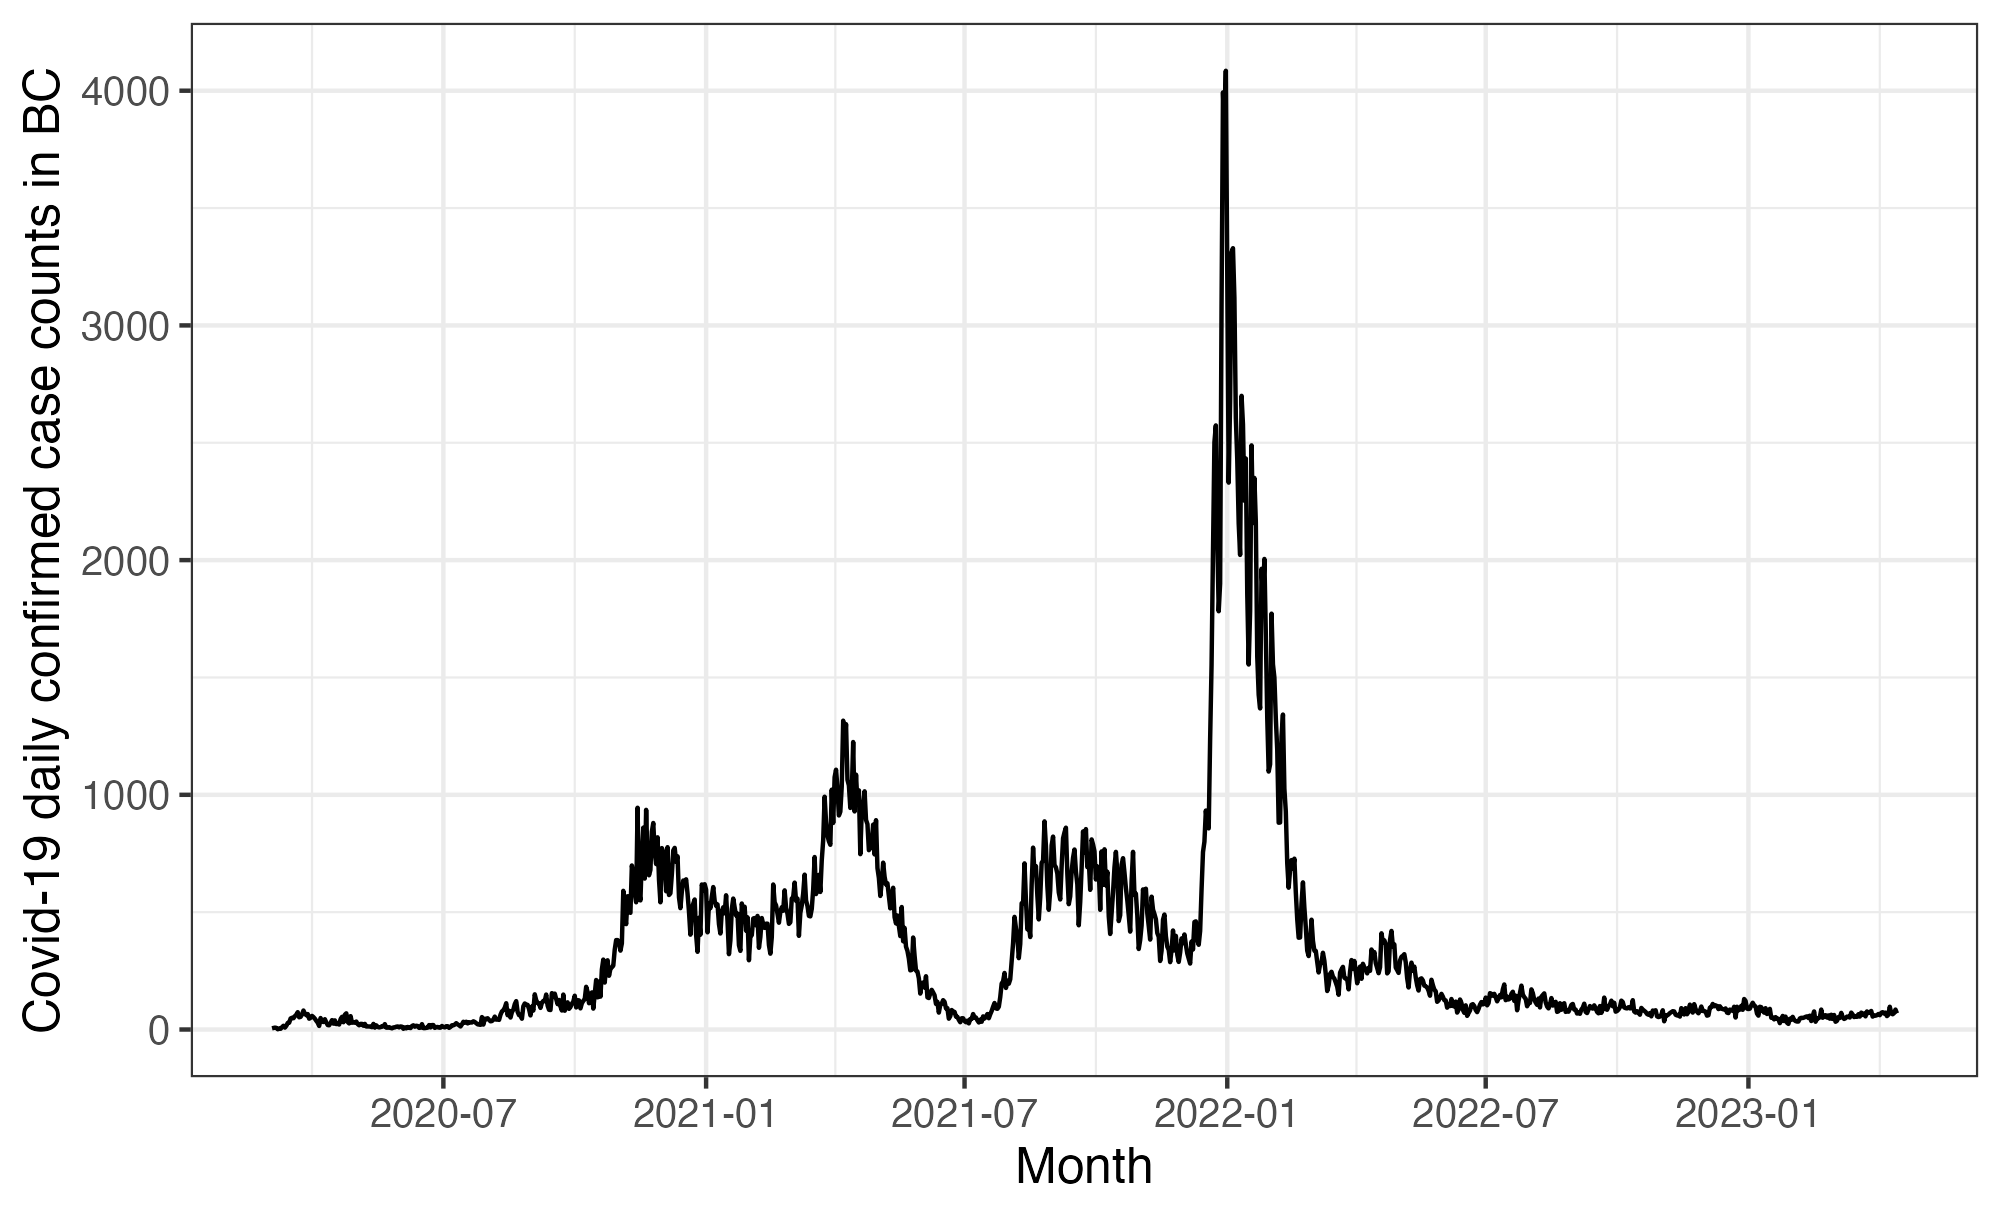
\includegraphics[width=0.99\linewidth]{fig/covid_dat.png}
    \caption{Covid19 daily confirmed incidence counts between March 1st, 2020 and April 15th, 2023 in British Columbia, Canada.} 
    \label{fig:covid-data}
\end{figure} 

% interpret figures -- across all lambdas
Considering the temporal evolutions of effective reproduction numbers across $3, 4, 5$ days, the estimated reproduction numbers of Covid-19 in British Columbia (illustrated in \autoref{fig:covid-rt}) are less than $3$ during most of the time, which means that one distinct infected individuals can on average infect less than three other individuals in the population. The three degrees of the temporal evolution (across all regularization levels $\lambda$) all yield similar results that $\hat{\calR}_t$ comes to the highest peak around the end of 2021 and then drops down to the lowest trough shortly thereafter. Throughout the estimated curves, the peaks and troughs of the reproduction numbers roughly come prior to the following growths and decays of confirmed cases respectively.
% CBs for real epidemic applications
We also visualize the 95\% empirical confidence bands of the point estimates for the ``best'' tuning parameter (in terms of MSEs). 

The reproduction numbers are relatively unstable before April 1st, 2022. The highest peak coincides with the emergence and globally spread of the Omicron variant. The estimated reproduction numbers are apparently below the threshold $1$ during two time periods -- roughly from April 1st, 2021 to July 1st, 2021 and from January 1st, 2022 to April 1st, 2022. The first trough coincides with the first authorization for use of Covid-19 vaccines in British Columbia. The second trough shortly after the greatest peak may credit to many aspects, including self-isolation of the infected individuals and application of the second shot of Covid-19 vaccines. Since around April 1st, 2022, the reproduction numbers stay stable (fluctuating around $1$) and the infected cases stay low. 

% for different lambda
Greater regularization levels (by using larger $\lambda$s) result in smoother estimated curves. Smoother curves suggest that the estimated reproduction numbers are around $1$ during most time periods; however, it may miss to capture some outbreaks of the pandemic. More wiggly curves better reflect the fluctuation of $\calR_t$, but sometimes fail to highlight the significant peaks or troughs. The tuning parameter $\lambda$ needs to be chosen corresponding to the information in practice for a better interpretation. Here, we provide the CV-chosen $\calR_t$ estimates with confidence bands. 
\begin{figure}[tb]
    \centering
    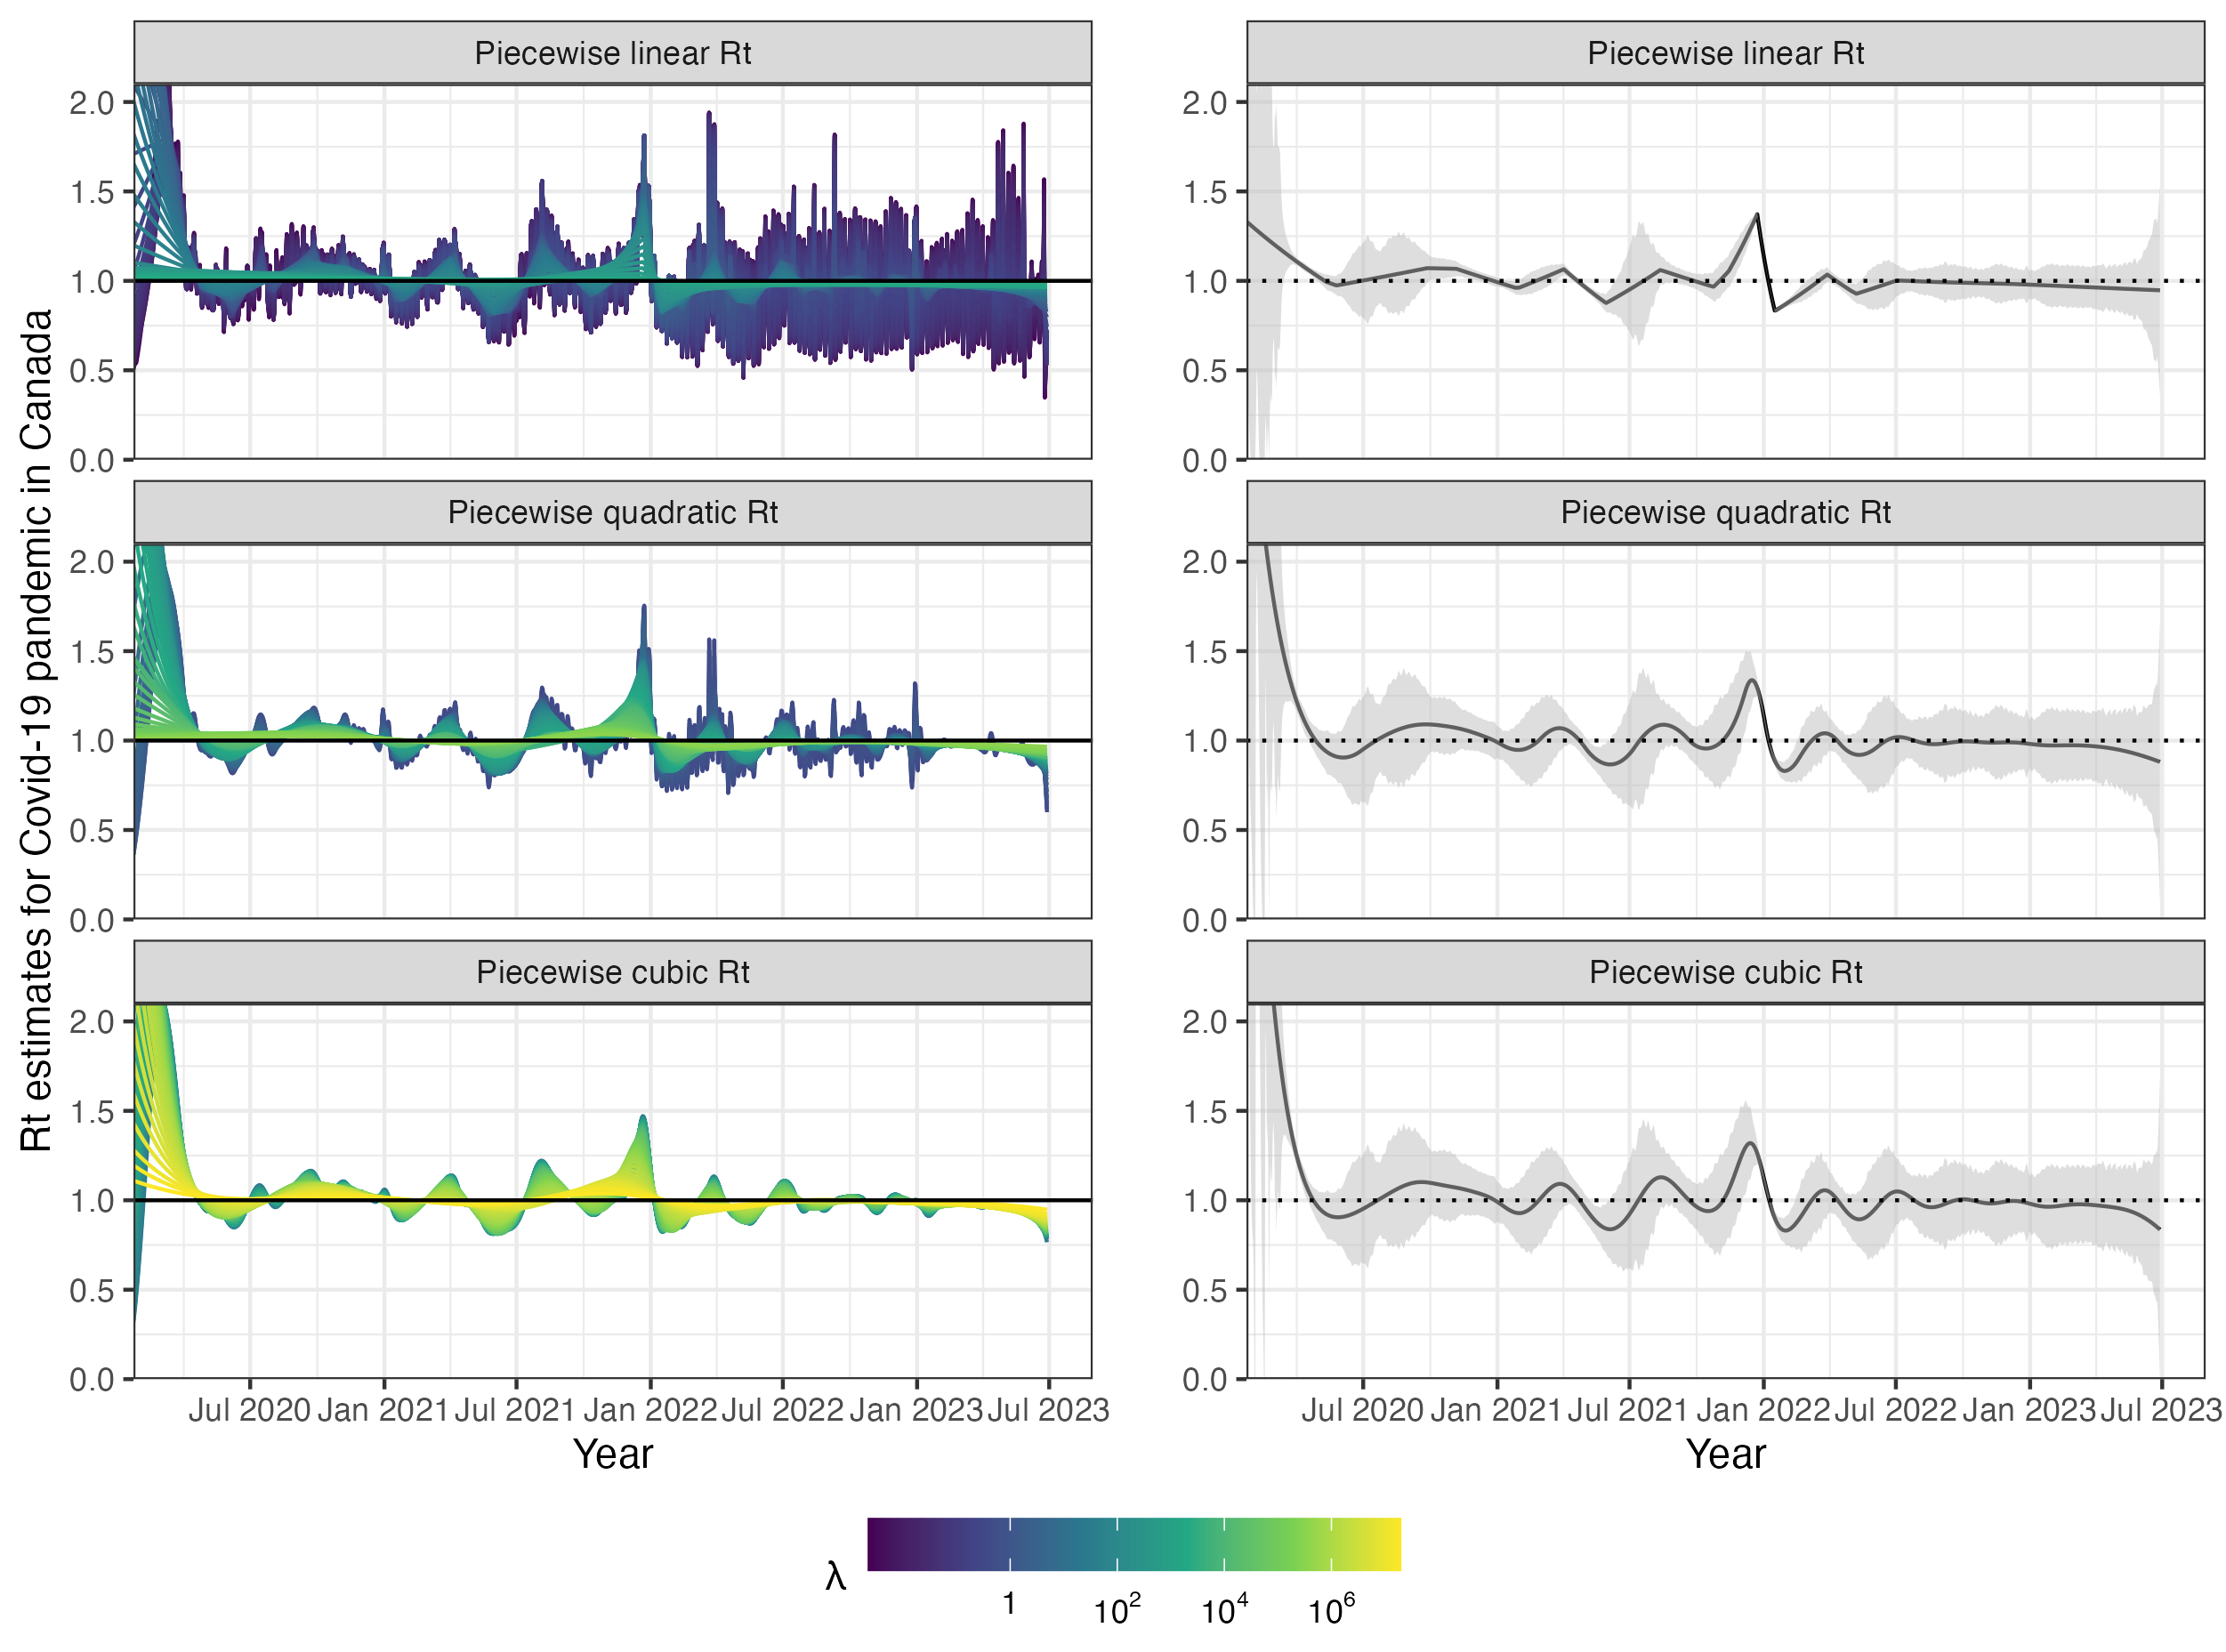
\includegraphics[width=0.99\linewidth]{fig/covid_full_res.png}
    \caption{Estimated effective reproduction numbers for Covid19 daily confirmed counts between March 1st, 2020 and April 15th, 2023 in British Columbia, Canada. The left panels display the CV-tuned estimates with 95\% confidence intervals. The right panels demonstrate estimates corresponding to 50 tuning parameters. The top, medium and bottom panels illustrate the estimated reproduction numbers ($\calR_t$) using the Poisson trend filtering (in \eqref{eq:rt-ptf}) with degrees $k=1,2,3$ respectively.} 
    \label{fig:covid-rt}
\end{figure} 


\subsection{Pandemic influenza in Baltimore, Maryland, 1918}

We then apply \RtEstim\ on the pandemic influenza in Baltimore, Maryland, 1918. Dataset in \autoref{fig:flu-dat} is obtained from the \texttt{R} package \EpiEstim. The 1918 influenza, caused by H1N1 influenza A virus, was an unprecedentedly deadly influenza that infected almost one-third of the population across the world \citep{taubenberger20061918}. 
In the estimation displayed in \autoref{fig:flu-res}, the CV-tuned piecewise cubic estimates better capture the growing tendency at the beginning of the pandemic. It suggests that the pandemic has yielded a decrease after around 20 days and reached $1$ when the pandemic has lasted for nearly 50 days. However, it also suggests an increase at the end of the period, while a steady decline (as in CV-tuned piecewise constant and linear estimates) is more reasonable. The smoothness of $\calR_t$ curves should be chosen based on the purpose of the study in practice, e.g., epidemic forecasting may require a more wiggly curve that contains more fluctuation information, while retrospective studies that solely target on understanding of the pandemic may prefer a smoother curve with less important information smoothed out. 
\begin{figure}[tb]
    \centering
    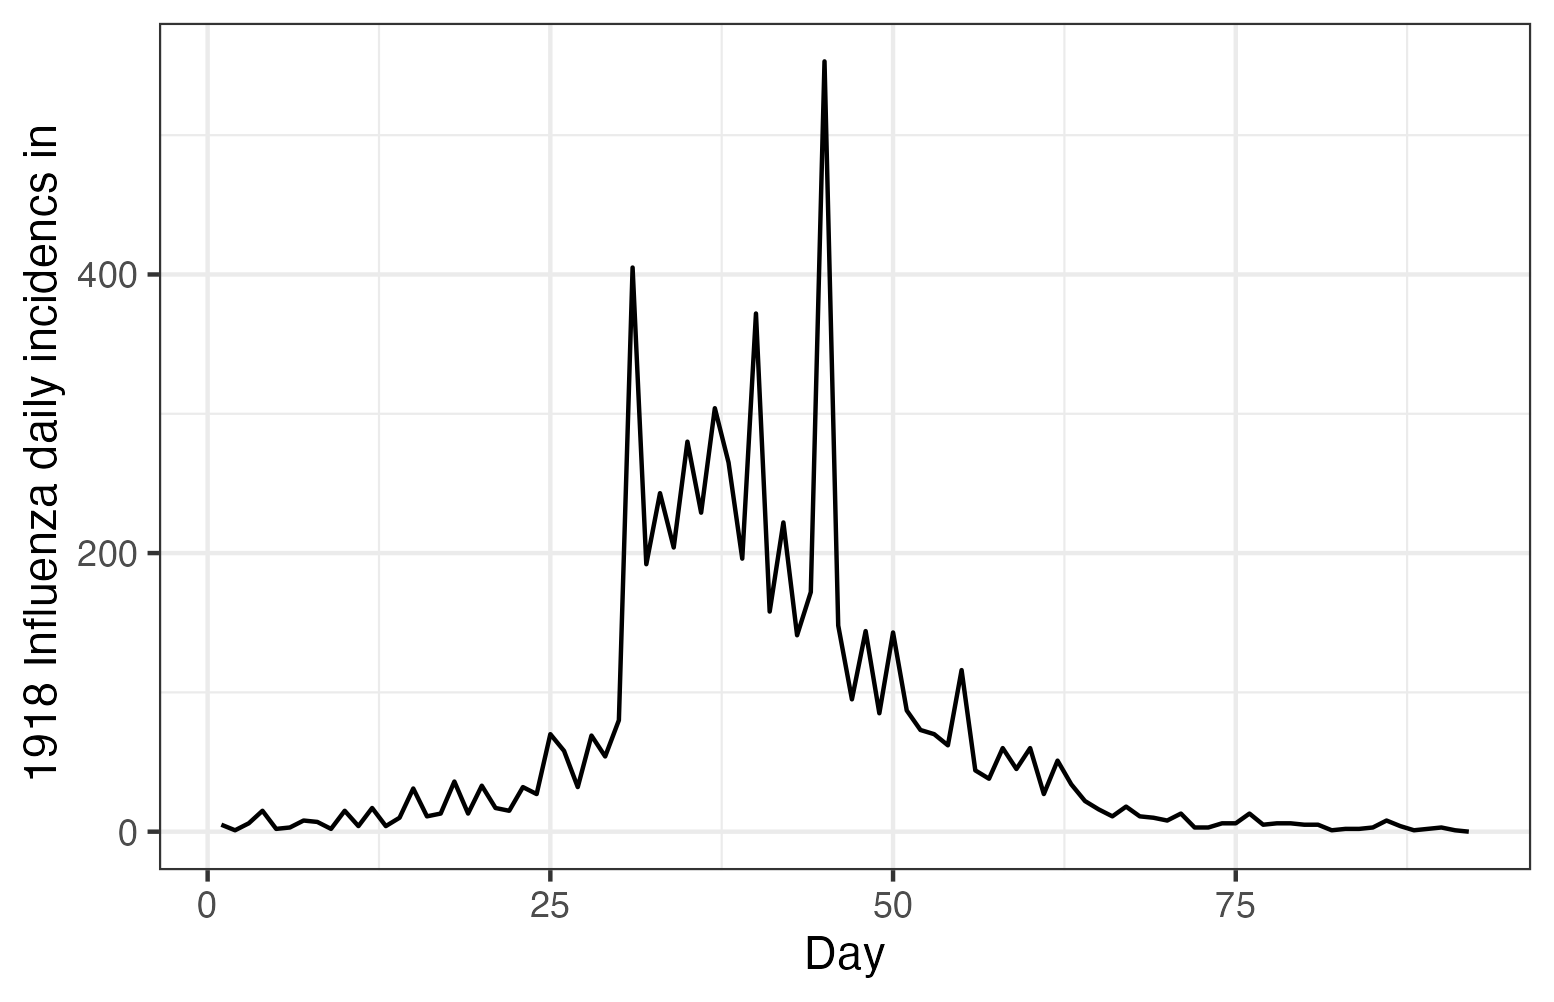
\includegraphics[width=0.9\linewidth]{fig/flu_dat.png}
    \caption{Pandemic influenza incidence counts in Baltimore, Maryland in 1918.} 
    \label{fig:flu-dat}
\end{figure} 

\begin{figure}[tb]
    \centering
    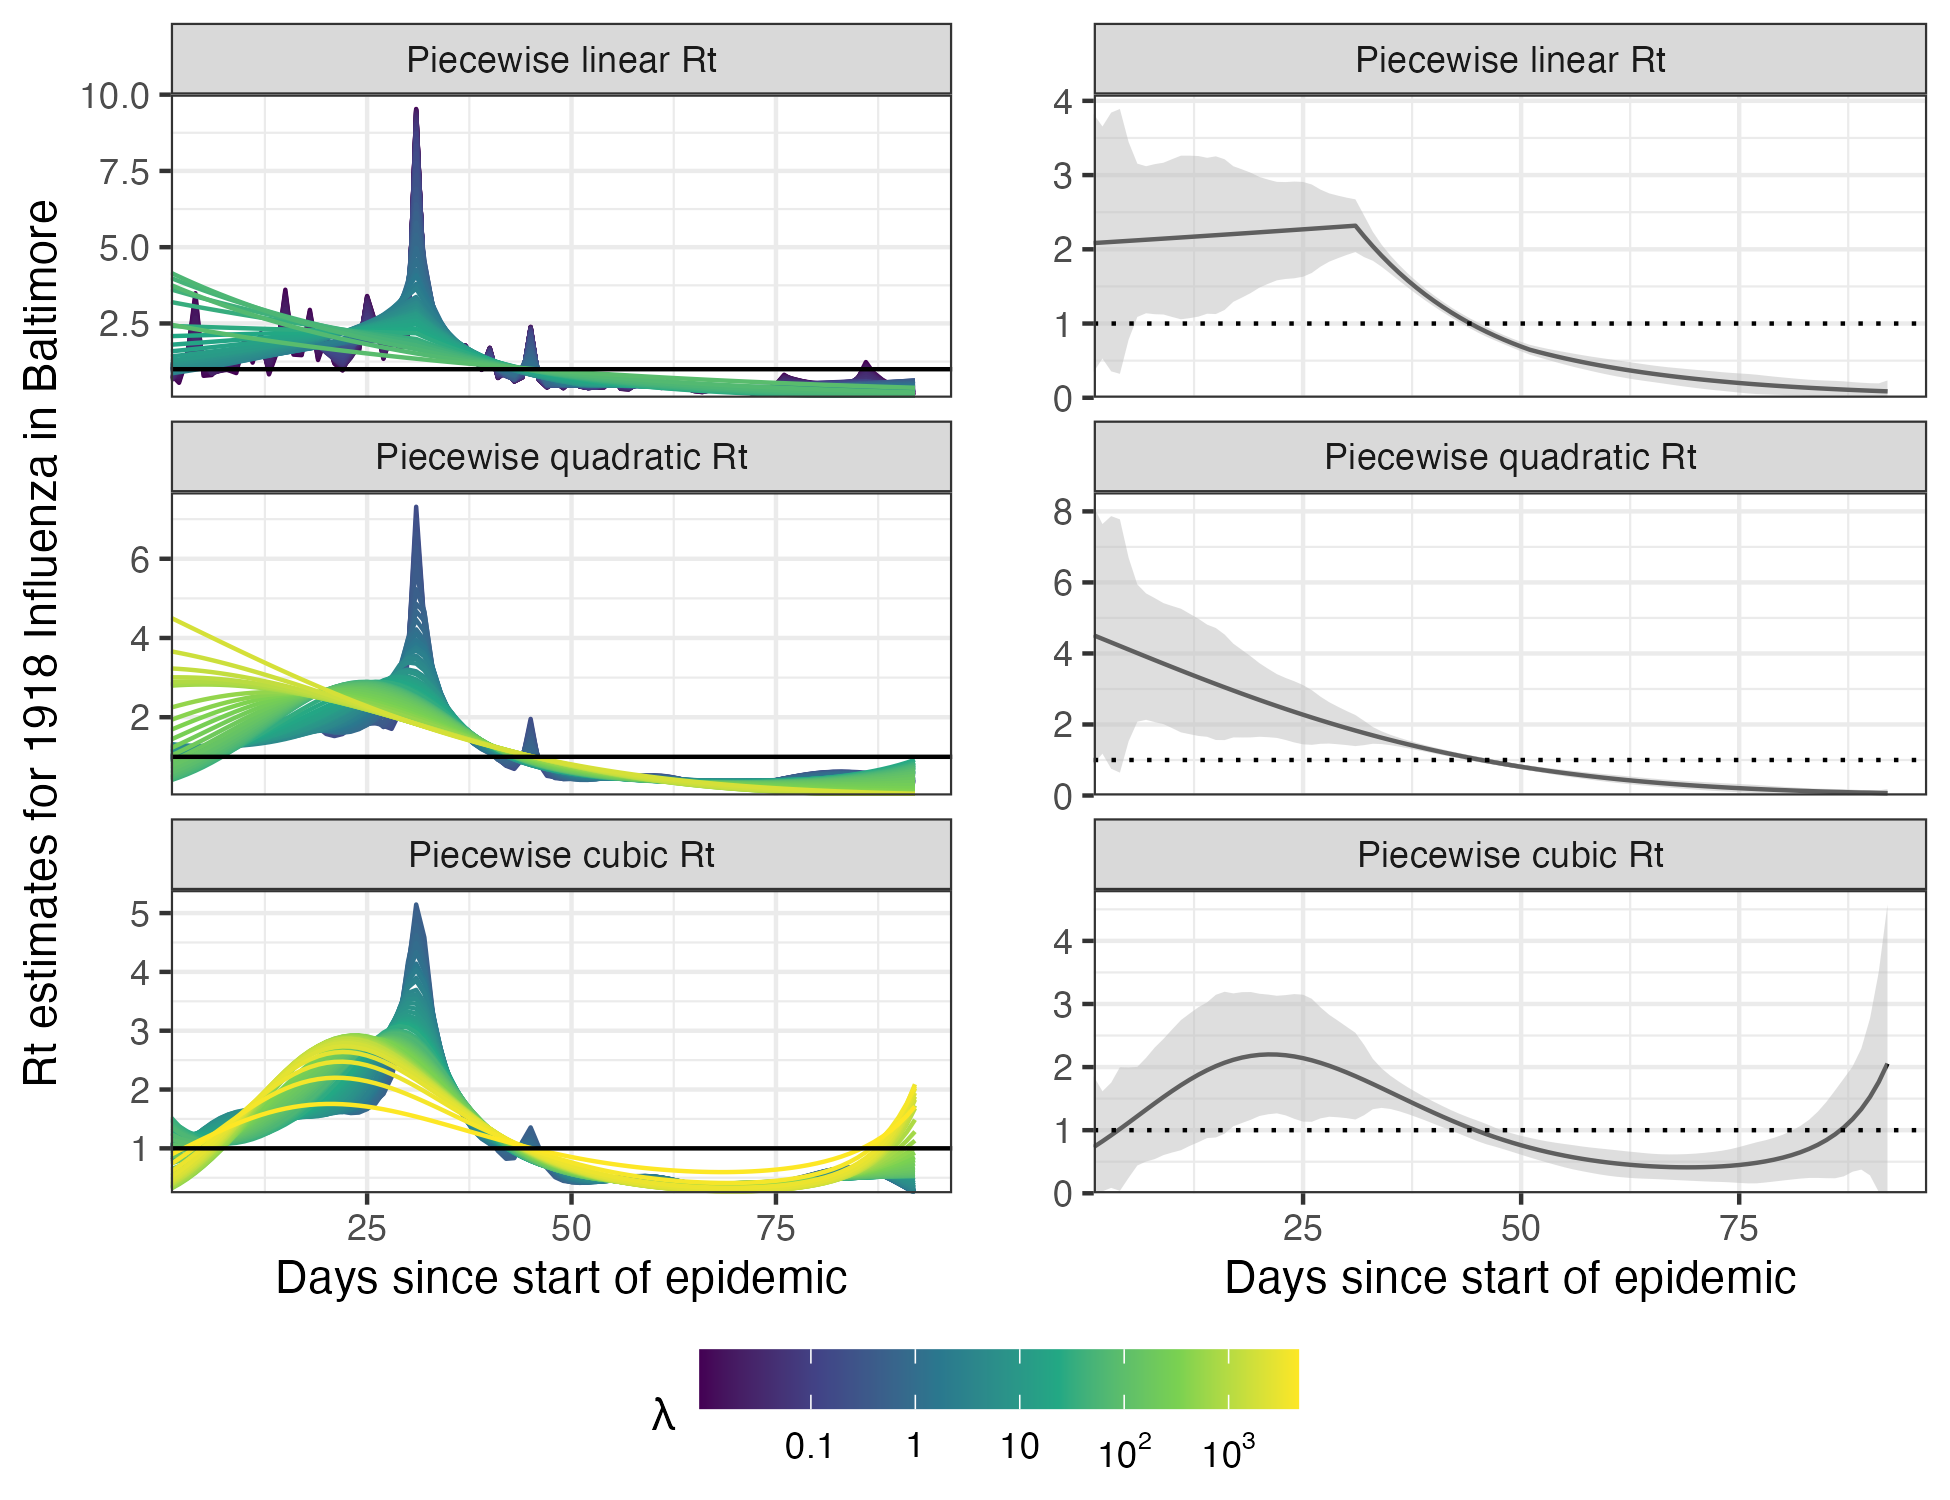
\includegraphics[width=0.9\linewidth]{fig/flu_full_res.png}
    \caption{Estimated effective reproduction numbers for pandemic influenza incidence counts in Baltimore, Maryland in 1918. The left panels display the CV-tuned estimates with 95\% confidence intervals. The right panels demonstrate estimates corresponding to 50 tuning parameters. The top, medium and bottom panels illustrate the estimated reproduction numbers ($\calR_t$) using the Poisson trend filtering (in \eqref{eq:rt-ptf}) with degrees $k=1,2,3$ respectively.} 
    \label{fig:flu-res}
\end{figure} 

